\chapter{Background}
\section{Early Computing}

\subsection{Pressey's Teaching Machines}

\par The concept of ``Learning Machines'' are actually older than Turing machines\footnote{We use the definition of ``Learning Machines'' provided in \cite{benjamin1988history}. That is, a teaching machine is an automated device that provides questions to the user and automatically grades them.}. The earliest learning machine was patented by Sidney L. Pressey in 1928 (See \textbf{\hyperref[fig:pressey_machine]{Figure \ref*{fig:pressey_machine}}}) \cite{benjamin1988history}. This machine was designed for both \textit{testing} and \textit{teaching}. In \textit{testing} mode, it would only give the user one chance to answer each question, but in \textit{teaching} mode the user could try as many times as they liked. After answering a specified number of questions correctly, the machine would dispense a piece of candy. The machine came equipped with a ``reward dial'' that allowed the researcher to define how many questions the user had to respond to before they earned the candy.

\par Unfortunately, Pressey was not able to find a market for his teaching machines. Skinner would later argue that it was the general culture of the 1920s and 30s that stopped Pressey's machines from gaining popularity; it wasn't until the 1950s and 60s where novel technology was more readily accepted into the mainstream \cite{skinner1958teaching}.

 \begin{figure}[h]
 	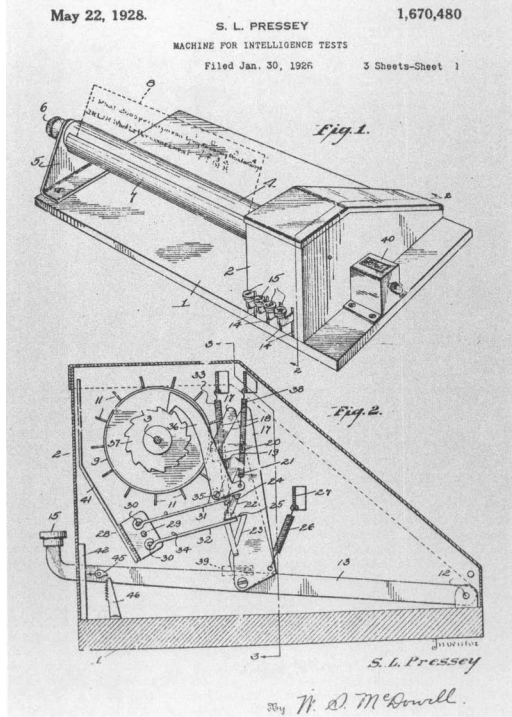
\includegraphics[width=1.0\linewidth]{figures/pressey_machine}
 	\caption{A diagram depicting the patent for Sidney Pressey's teaching machine. Candy was dispensed to the user after answering a question correctly.}
 	\label{fig:pressey_machine}
 	\cite{benjamin1988history}
 \end{figure}
 
 \subsection{Skinner's Teaching Machines}
 \par Dr. B. F. Skinner continued the work of Pressey. In 1958, he published a paper describing his newer teaching machine based off punchcard computing technology. While using Skinner's machine, students receive a rotation of questions about a certain subject, and could not continue until they had answered each question in the rotation correctly. The cycle of questions presented the information in varied ways. For instance, in \textbf{\hyperref[fig:skinner_machine]{Figure \ref*{fig:skinner_machine}}}, a series of questions that teach the student how to spell ``manufacture'' is displayed. The first question simply asked the student to repeat the word, and the rest of the questions transform that question in various ways, which Skinner hoped would ``hold the student's attention'' and force them to process the information in different ways, accelerating the learning process. 
 
 \begin{figure}[h!]
 	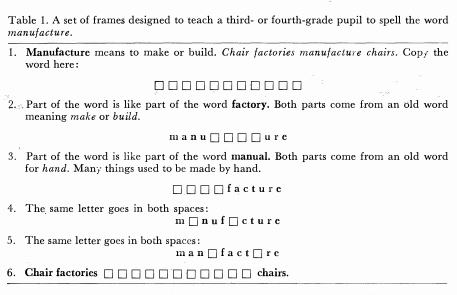
\includegraphics[width=1.0\linewidth]{figures/skinner_machine}
 	\caption{A series of questions as presented by Skinner's teaching machine. The question is ``transformed'' to several different modes that help the user learn the information faster. }
 	\label{fig:skinner_machine}
 	\cite{benjamin1988history}
 \end{figure}
 

\par Dr. Skinner believed that computers would completely revolutionize classrooms. Students would be able to learn at their own pace, with the computer determining the optimal schedule for each student based on how they were performing. Skinner made it clear that he didn't envision his computers as replacing human teachers, but rather supplementing their teaching, saving them time and making learning a more efficient process.

\subsection{Behavior and Learning}

Of course, B. F. Skinner is most famous for his creation of the ``Skinner Box,'' \cite{skinner1963operant} a device that gave simple reinforcement to animals or humans in the lab in order to slowly shape their behavior, through a process known as operant conditioning. When a subject performed well according to the test, they would receive a small reward, while if they strayed from the purpose of the test, they would not receive a reward. Dr. Skinner argued that ``much of what we know [about the learning process] has come from studying the behavior of lower organisms, [and] the results hold surprisingly well for human subjects'' \cite{skinner1958teaching}. Skinner's research hearkens back to the candy that was dispensed by the early teaching machines of Pressey.

\par It's important to note the connection between operant condition and learning. Skinner believed that learning was simply a form of behavior modification, and that 

% TODO: Define behavior, tie it in to learning, tie it into habits.
\par 


\subsection{Variable Ratio Reinforcement Scheduling}
 Behavior modification can be accelerated through the use of \textit{variable ratio reinforcement scheduling }\cite{ferster1957schedules}. There are several different ways of scheduling the rewards  where rewards are not actually doled out on a regular basis exactly according to the behavior of the test subject. Instead, rewards are handed out semi-randomly, varying in quantity and quality, while still mostly rewarding the desired behavior that the researcher is trying to condition. This causes the test subject to become conditioned much faster (See \textbf{\hyperref[fig:variable_ratio]{Figure \ref*{fig:variable_ratio}}}).
 
 \begin{figure}[h]
 	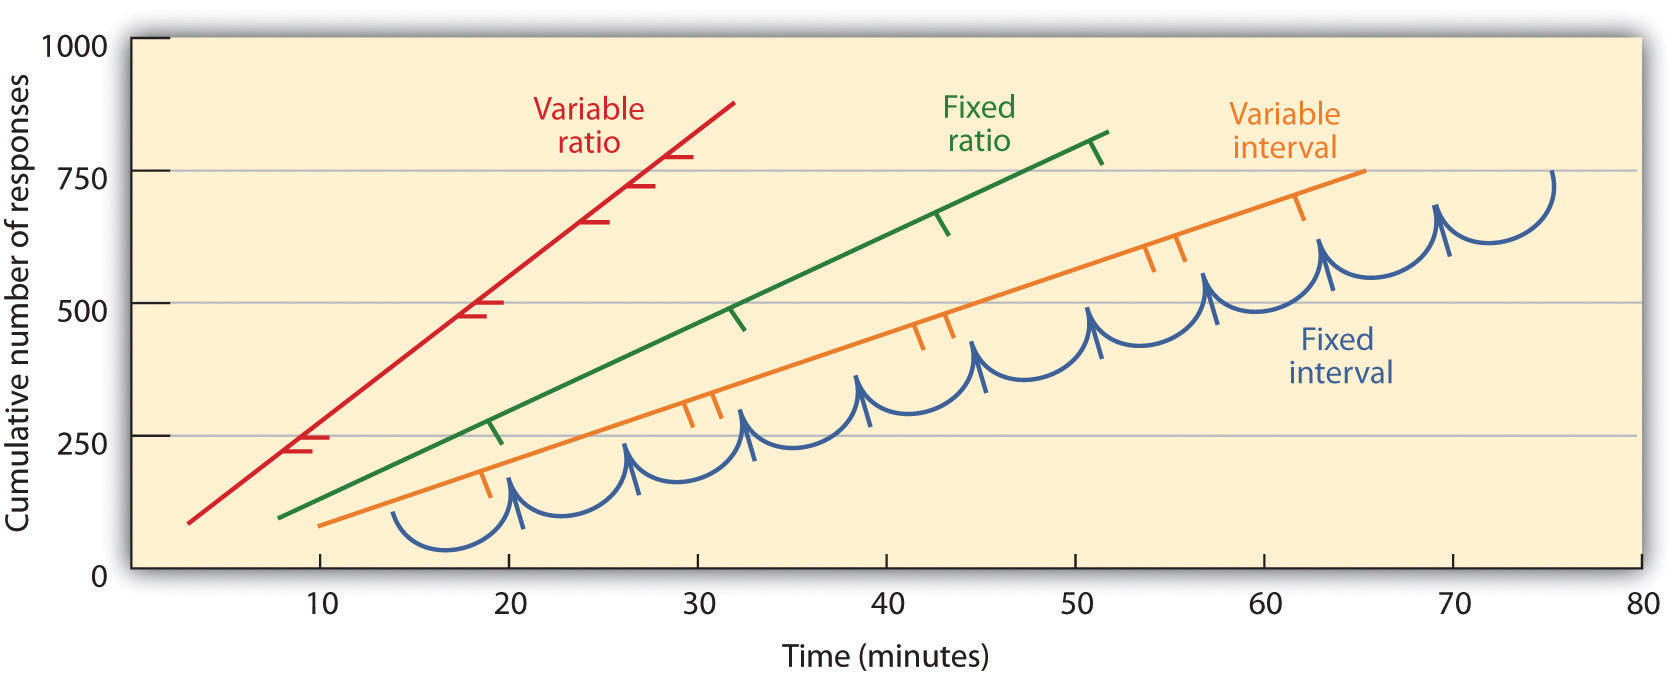
\includegraphics[width=1.0\linewidth]{figures/variable_ratio}
 	\caption{Variable ratio rewards scheduling. Note that as rewards are spaced out randomly, the desired behavior appears much more quickly.}
 	\label{fig:variable_ratio}
 	\cite{hardy_heyes_1999}
 \end{figure}

\section{Habit Formation}



The study on Duolingo notes how difficult it is to actually get people to use the app. It is extremely hard to change people's habits, taking a lot of time and effort on the user's part to effectively change their behavior. One such strategy around this is to connect one desired ``habit'' behavior to an existing habit \cite{lally2010habits}. For instance, test subjects in the study by Dr. Lally determined that it was easiest to condition subjects to perform some action by instructing them to perform it right after eating breakfast in the morning. By using the powerful force behind an existing habit, it is possible to ``reprogram'' your behavior such that a new habit is formed with the new desired behavior.

For instance, if a subject wants to make a habit of cleaning their room, they can make a habit of picking up one piece of clothing after coming home from work for the day. In this way, the habit is driven forward by the regular schedule of coming home at a regular time each day. By associating one behavior with an existing behavior, it is possible to rewire a subject's brain to complete the second behavior far more often.

% TODO Need to read this paper + book in-depth and get a good idea of how habit forming applications go down.
\subsection{New Psychological Theories}
It's interesting to note that the advent of ``apps'' and habit-forming application has created an essentially new field in psychology \cite{renfree2016don}. In a study, Dr. Renfree argues that the behavior modifications seen in apps like Lift and Memrise actually represent new advances into how habit-forming psychology operates.

% TODO Also expand on this part. The DARK SIDE of gamification, yo
Unfortunately, most of these new effects are actually negative. For instance, Dr. Renfree notes that oftentimes the new habits generated by these apps are ``fragile,'' since they are so dependent on a tight dopamine-based reinforcement loop. As soon as the loop is broken, the brain ``loses interest'' and the new 
information is deprioritized. This will be an interesting consideration as we develop our application. We want to ensure that the habits and knowledge developed by our app is not simply impermanent, and that it won't be simply ``pushed out'' by new information.




% TODO: Why is this here? Shouldn't it be in related works
\section{Duolingo}
As mentioned previously in the introduction, Duolingo is an app that already uses several of the processes that we are describing. Duolingo has been shown to be very effective for learning new languages, even perhaps more effective than typical classes. However, the effectiveness of Duolingo is mostly contingent on the motivation of the student. If the student is going to a foreign country soon, Duolingo is the most effective since there is a significant time pressure and pressure to learn the language in order to fit in at whatever country the student is planning to go to \cite{vesselinov2012duolingo}. If, however, the student is simply learning another language for fun, there will be significantly less benefit to them. We must consider this as we develop our educational software; apparently the nature of the student's motivation and their reason for wanting to learn the subject material plays heavily into wheter or not they will be successful in using the app.